\documentclass[FM,ZP]{tulthesis}
\usepackage[czech]{babel}
\usepackage[utf8]{inputenc}
\usepackage{pdfpages}
\usepackage{graphicx}
\usepackage{tikz}
\usepackage{url}
\usepackage{float}  % Ukotvení věcí na svém místě (obrázky, tabulky, grafy, ...)
\usepackage{hyperref}  % Klikací odkazy v obsahu a referencích

\TULtitle{Případová studie - Analýza celosvětových prodejů počítačových her}{}
\TULprogramme{N2610}{Elektrotechnika a informatika}{Electrical Engineering and Informatics }
\TULbranch{1802T007}{Informační technologie}{Information Technology}
\TULauthor{Bc. Tomáš Moravec}
\TULsupervisor{}
\TULacad{2016/2017}

\begin{document}
\ThesisTitle{CZ}
\renewcommand{\baselinestretch}{1.50}
\setlength\parindent{1.2cm}
\selectfont
	
\begingroup
\renewcommand{\cleardoublepage}{}
\renewcommand{\clearpage}{}
\chapter{Zadání}
\endgroup
Pomocí více než 16 500 záznamů, z největší celosvětové databáze prodejů počítačových her VGChartz se pokusím analyzovat, jaký je klíč k vydání úspěrné hry pro jednotlivé kontinenty, případně jak se trendy měnily v průběhu posledních let.
	
\begingroup
\renewcommand{\cleardoublepage}{}
\renewcommand{\clearpage}{}
\newpage
\chapter{Zdrojová data}
\endgroup

\section{Získání dat}
Data ke zpracování vybrané úlohy, tedy analýza celosvětových prodejů počítačových her, jsem se rozhodl hledal na největších data-miningových portálech, zejména jsem procházel UCI, Kaggle a KDNNuggets. Konečná zdrojová data jsem si vybral z portálu Kaggle (jedná se o projekt společnosti Google, nyní již Alphabet Inc.), přesněji na adrese \url{https://www.kaggle.com/gregorut/videogamesales}, kde jsem nalezl největší množství dat ke zpracování. Zdrojem dat je portál VGChartz a získána byla pomocí scrape bota, dostupného na adrese \url{https://github.com/GregorUT/vgchartzScrape}.

\section{Struktura dat}
Data obsahují jak globální prodeje, tak prodeje na jednotlivých trzích. Do tabulky se dostali pouze hry, které měli více než 100 000 prodaných kopií.

\paragraph{Přesněji jsou data strukturovaná takto:}
\begin{itemize}
\item Rank - Pořadí v tabulce
\item Name - Celý název hry
\item Platform - Platforma (zařízení), pro které hra vyšla (PC,PS4, atd.)
\item Year - Rok vydání hry
\item Genre - Herní žánr
\item Publisher - Vydavatelství hry
\item NA\_Sales - Prodeje v Severní Americe (v milionech)
\item EU\_Sales - Prodeje v Evropě (v milionech)
\item JP\_Sales - Prodeje v Japonsku (v milionech)
\item Other\_Sales - Prodeje ve zbytku světa (v milionech)
\item Global\_Sales - Prodeje celosvětově (v milionech), jedná se o součet ostatních
\end{itemize} 

\begin{figure}[H]
\begin{center}
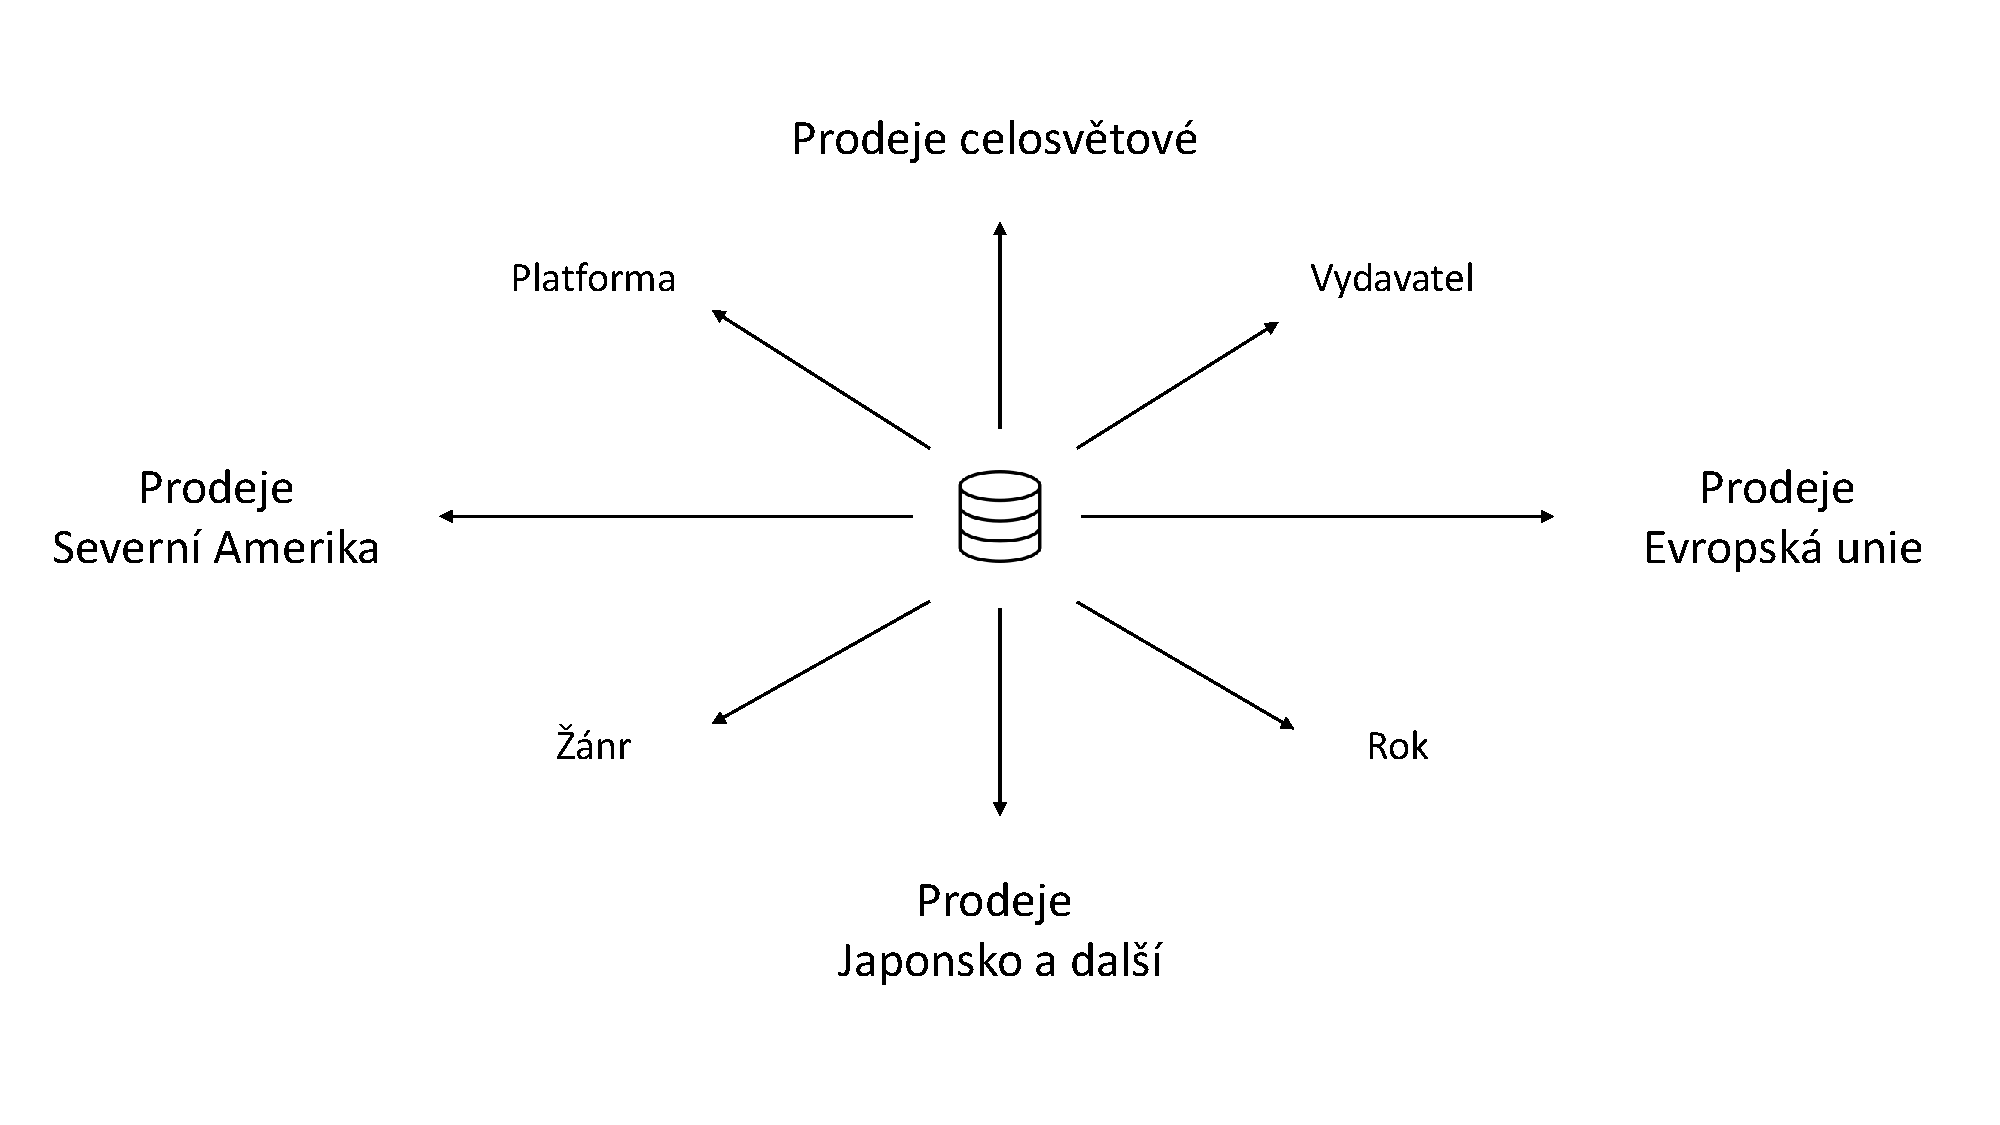
\includegraphics[width=\textwidth]{images/dataStructure.pdf}
\caption{Grafické znázornění dat}
\label{image}
\end{center}
\end{figure}

\chapter{Příprava dat}

V tomto příkladu budeme pracovat s dodanou datovou maticí. Je však třeba ověřit kvalitu dat a analyzovat rozdělení jednotlivých proměnných.

\section{Zlepšení kvality dat}
Po bližším prozkoumání dat jsem zjistil, že valná většina dat je velice nekvalitních. Pro prozkoumání jednotlivých nekvalitních záznamů a několika méně úspěšných pokusech o zlepšení kvality jsem přišel na to, že pokud omezím rok vydání, na období, ve kterém jsou vydávány všechny moderní hry, tedy od roku 1980 (Wikipedia) do dnes, tedy do roku 2017, data získají 100\% kvalitu. Po prozkoumání již kvalitních dat jsem došel k pouhým 2 121 záznamům. Postup je znázorněn na obrázku níže.

\begin{figure}[H]
\begin{center}
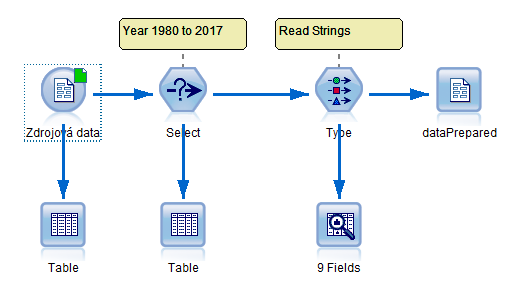
\includegraphics[width=0.9\textwidth]{images/dataPreparation.png}
\caption{Postup výběru kvalitních dat}
\label{image}
\end{center}
\end{figure}

\chapter{Vyhodnocení dat}

\section{Rozdělení na období prodejů}
Prvním úkolem bylo, zvolit si správné období tak, aby bylo možné vidět nejenom aktuální dění na herním trhu, ale také proměnu trhu v posledních letech. Zvolil jsem si období prodejů za 1 poslední rok (2016 a začátek 2017) a dále za 5 posledních let (2011 až začátek 2017). Data obsahují i několik her z ledna 2017, která jsem započítal do roku 2016.

\begin{figure}[H]
\begin{center}
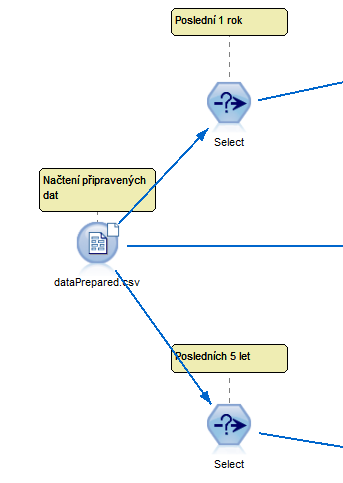
\includegraphics[width=0.5\textwidth]{images/separation.png}
\caption{Rozdělení dat na zvolená období}
\label{image}
\end{center}
\end{figure}
	
\section{Zpracování jednotlivých období}
Jednotlivá období jsem zpracovával identicky, zaměřím se tedy pouze na poslední 1 rok. Rozhodl jsem se zjistit, jak zisky ovlivňují platformy, vydavatelství a žánr hry.

\subsection{Celosvětové prodeje v závislosti na platformě}
Nejdříve jsem se zaměřil na získání informací o globálních zisků z jednotlivých platforem, tedy zařízení, pro které probíhal vývoj hry a na které si jí lze zahrát.

\begin{figure}[H]
\begin{center}
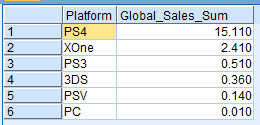
\includegraphics[width=0.4\textwidth]{images/platformSales.png}
\caption{Tabulka celosvětových prodejů pro jednotlivé platformy za poslední rok}
\label{image}
\end{center}
\end{figure}

Z tabulky je patrné, že dnes nejpopulárnější platformy jsou ty nejvýdělečnější. 

\subsection{Celosvětové prodeje v závislosti na vydavatelství}
Dále jsem se tedy zaměřil na samotná vydavatelství, která za vývojářské studio vydávají hru, stejně jako knižní vydavatelství vydává hru za spisovatele. Zajímalo mě tedy, zda jsou zisky ovlivněny výběrem vydavatelství.

\begin{figure}[H]
\begin{center}
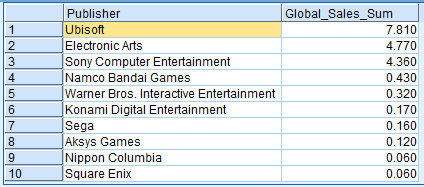
\includegraphics[width=0.75\textwidth]{images/publisherSales.png}
\caption{Tabulka celosvětových prodejů pro deset největších vydavatelství za poslední rok}
\label{image}
\end{center}
\end{figure}

Není překvapivé, že největší vydavatelství, které mají největší distribuční sítě, dokáží hře vygenerovat značně vyšší zisky. Jedná se tedy o ekvivalent ke knižnímu vydavatelství.

\subsection{Celosvětové prodeje v závislosti na žánru hry}
Poslední zkoumanou kategorií je žánr hry, tedy zda se jedná o strategickou, sportovní, nebo jinou hru.

\begin{figure}[H]
\begin{center}
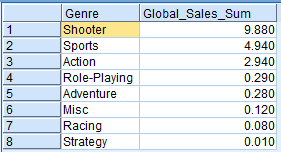
\includegraphics[width=0.45\textwidth]{images/genreSales.png}
\caption{Tabulka celosvětových prodejů pro jednotlivé žánry her za poslední rok}
\label{image}
\end{center}
\end{figure}

Ve výsledku jsem byl velice překvapen, že sportovní hry mají takovéto prodeje. Hlubším průzkumem jsem zjistil, že je to díly prodejům rodinných her, například pro Kinect, které ovládáte pohybem vlastního těla. Tyto hry jsou v posledních letech velice populární.

\subsection{Postup získávání jednotlivých výsledků}
Na obrázku níže je ukázáno, jak probíhalo získávání zobrazených dat.

\begin{figure}[H]
\begin{center}
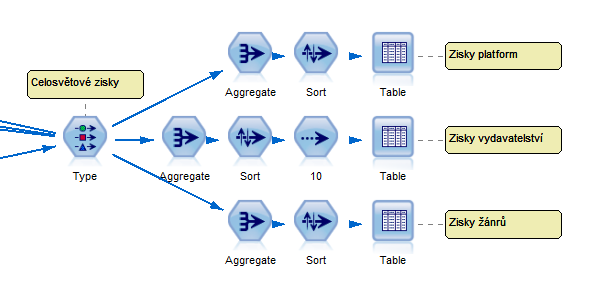
\includegraphics[width=0.9\textwidth]{images/oneYearParametres.png}
\caption{Získávání výsledků pro jednotlivé parametry}
\label{image}
\end{center}
\end{figure}

Na konci jsem ještě dělal průzkum vždy pro 3 největší vydavatelství (Sony, EA, Ubisoft), pro které platformy a žánry tvoří hry. Zda se drží nejvýdělečnějších, nebo se vymykají. Zjištění bylo takové, že největší vydavatelství striktně vydávají hry pouze na nejvýdělečnější platformy, stejně tak hry nejvýdělečnějších žánrů.

\section{Změny trhu}
Vhledem k tomu, že prozkoumávána byla data jak za poslední rok, tak za posledních 5 let. Došel jsem k následujícím výsledkům.

\subsection{Zisky z platform, vydavatelství a žánrů}
U platforem se v průběhu let nezměnilo v podstatě nic. Jednou za několik let vždy vychází modernější verze pro každou platformu, je tedy jasné že zisky za posledních 5 let jsou primárně ze starších verzí těchto platforem. Nicméně jiné rozdíly nejsou.

\begin{figure}[H]
\begin{center}
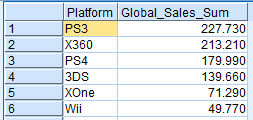
\includegraphics[width=0.4\textwidth]{images/fiveYearPlatform.png}
\caption{Získávání výsledků pro jednotlivé parametry za posledních 5 let}
\label{image}
\end{center}
\end{figure}

U ostatních parametrů (vydavatelství a žánr) se jedná o stejné výsledky. Tedy trendy se za poslední roky příliš nezměnily. Stejně tak největší vydavatelství vydávají pořád na největší platformy a vydávají hry primárně s nejprodávanějšími žánry.

\section{Vývoj zisků za všechna období}
Pro zajímavost jsem ke konci své práce prozkoumával historické vývoje zisků skrze všechna zaznamenaná období. Má očekávání byla, že prodeje budou každoročně růst, nebo stagnovat, nicméně, k mému překvapení, získal jsem naprostý opak.

\begin{figure}[H]
\begin{center}
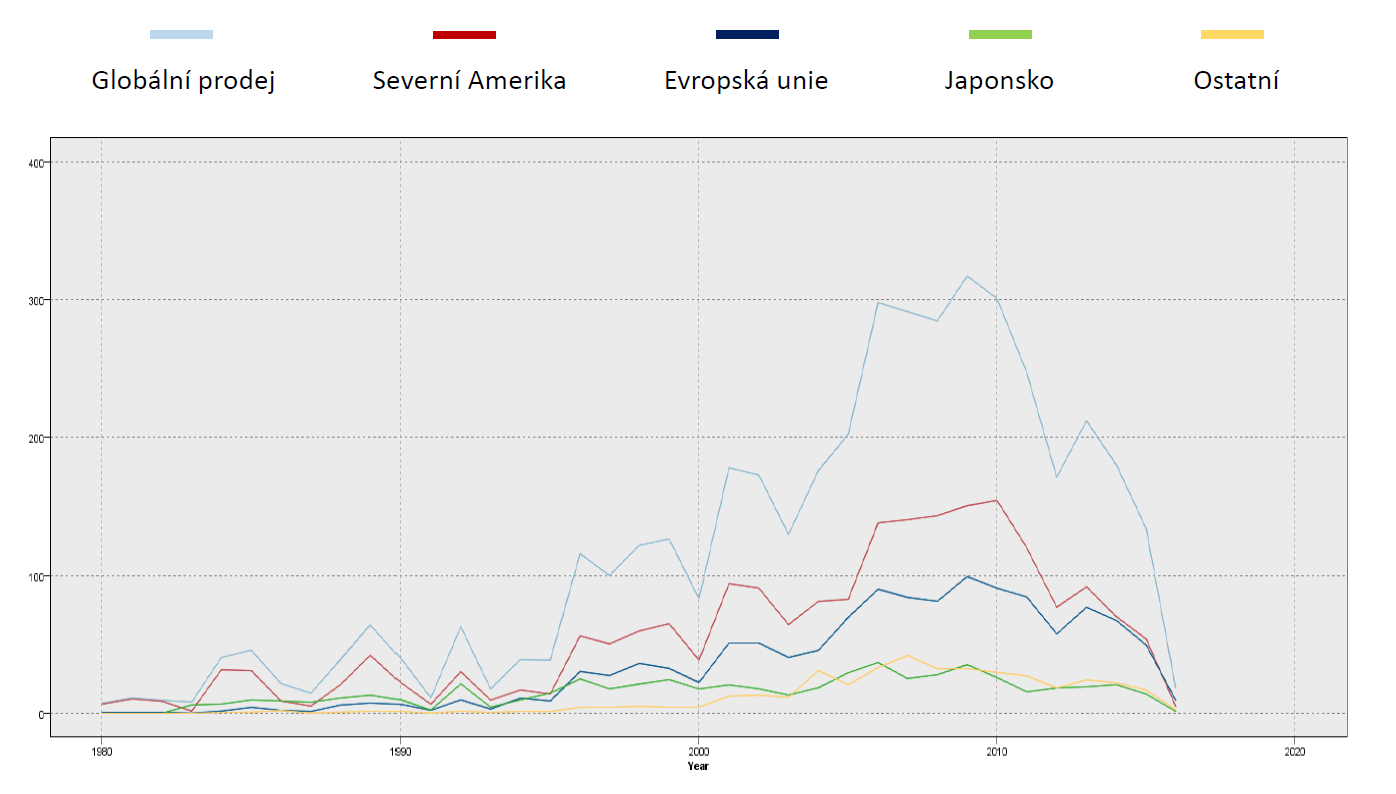
\includegraphics[width=\textwidth]{images/graphOfSales.png}
\caption{Vývoj zisků za všechna období}
\label{image}
\end{center}
\end{figure}

Ze získaných dat jsem byl zmatený, udělal jsem tedy analýzu závislosti prodejů na dvou nejvýdělečnějších platformách a na všech platformách, výsledky byli ale totožné. Níže je možné vidět postup při získávání grafů v závislosti na parametrech.

\begin{figure}[H]
\begin{center}
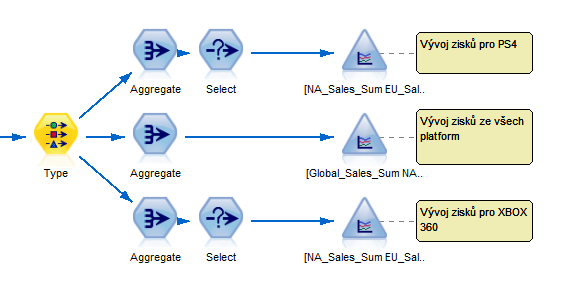
\includegraphics[width=0.9\textwidth]{images/alloverSales.png}
\caption{Zjištění vývoje zisků v závislosti na jednotlivých parametrech}
\label{image}
\end{center}
\end{figure}

Prohledal jsem, zda nemám chybu v postupu, kterou jsem neodhalil a vzhledem k totožným výsledkům jsem tedy závěrem považoval výsledky za správné, i když zvláštní. Vysvětlení přišlo až po prezentaci mé práce, viz závěr (nové skutečnosti), od jednoho ze studentů. Pro zajímavost přidávám vzhled kompletního proudu.

\begin{figure}[H]
\begin{center}
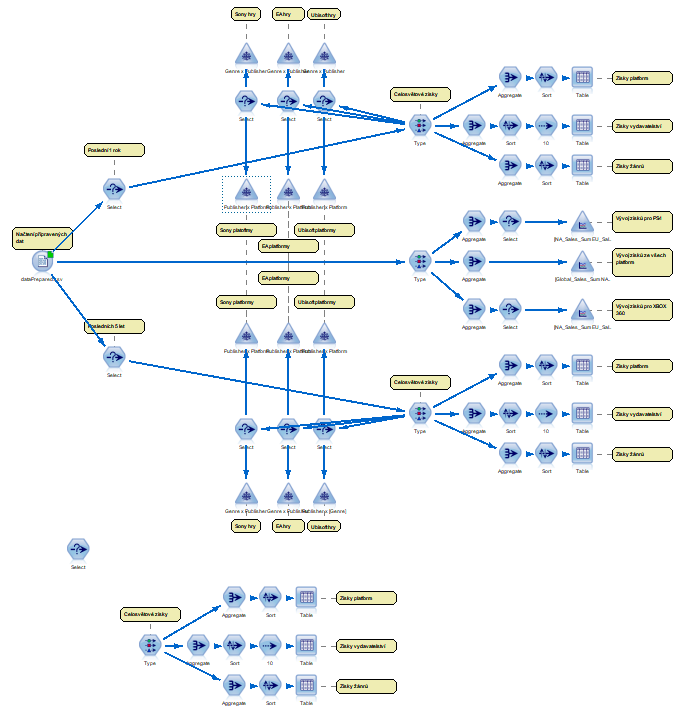
\includegraphics[width=\textwidth]{images/all.png}
\caption{Kompletní datový proud v modeleru}
\label{image}
\end{center}
\end{figure}

\chapter{Závěr}

\section{Shrnutí práce}
Výsledkem práce je, že pokud chcete maximalizovat možné zisky ze hry, je nutné využít jednoho ze tří největších distributorů her (Sony, EA, Ubisoft), dále je nutné se zaměřit na nejpopulárnější platformy (Playstation, Xbox) a zvolit poslední nejoblíbenější žánr (Akční, Sportovní). Myslím, že tyto skutečnosti byli pro člověka se zájmem o herní průmysl jasné již od začátku. Nicméně jsem byl velice překvapen z celosvětových prodejů, které jasně ukazovaly extrémní pád prodejů her. Důvod k takovýmto závěrům je vysvětlen v následujícím odstavci.

\section{Nové skutečnosti}
Po prezentaci mé práce na cvičení, mi bylo kolegou Karlem Šírem sděleno, že se o portál, ze kterého data čepají, zajímá a že prodeje jsou pouze z kamenných obchodů a chybí tedy největší distribuční sítě současnosti, jako je Steam, Origina a další. Bylo to pro mě na jednu stranu nečekané zjištění, na druhou stranu tato skutečnost objasnila, proč data ukazují extrémní úpadek prodeje her v posledních letech, trh se jednoduše adaptuje na prodeje online a kamenné obchody ztrácí na oblibě. Navazující práce na toto téma by mohla zahrnovat data ze všech prodejních sítí, díky čemuž bychom získali přesnější obraz o aktuálním dění na herním trhu.

\end{document}